\chapter{Results and Discussion}
\label{ch:results}

\section{Introduction}
This chapter reports the empirical evaluation of Synergy-FedFM. The objective is to demonstrate that high-performance anomaly detection can be maintained at the extreme edge while substantially reducing communication overhead. The evaluation proceeds in three stages: (1) establish a centralized Oracle baseline trained on the full dataset; (2) perform a systematic hyperparameter sweep using Latin Hypercube Sampling (LHS) across quantization, coreset size, low-rank adaptation (LoRA), and novelty threshold; and (3) identify Pareto-optimal configurations that trade cumulative compression ratio (CCR) against accuracy degradation ($\Delta F1$).

All experiments use a CICIDS2017-derived dataset partitioned across simulated clients. Macro F1 is reported as the primary accuracy metric, and federated performance loss is defined as $\Delta F1 = F1_{\text{oracle}} - F1_{\text{federated}}$. The Pareto frontier is constructed from aggregated results in \texttt{results/lhs_summary.csv} and visualized in Figure~\ref{fig:pareto_frontier}.

\section{Establishing the Centralized Oracle Baseline}
The centralized Oracle represents the practical performance upper bound: a model trained on the entire dataset (N = 223,082 samples) with class-balanced training procedures. For rigorous comparison, the Oracle F1 was measured on the same held-out test partition used throughout the federated experiments. The verified Oracle macro F1 is $0.9257$, and this value is used as the fixed reference for all subsequent $\Delta F1$ calculations.

Anchoring federated measurements to a robust Oracle is essential: $\Delta F1$ quantifies the absolute degradation introduced by federated compression and communication constraints. Using a high-quality, stable Oracle eliminates variance due to repeated centralized retraining and enables fair comparison across heterogeneous LHS configurations.

\section{Hyperparameter Optimization via Latin Hypercube Sampling}
Latin Hypercube Sampling (LHS) was selected to efficiently explore the multi-dimensional hyperparameter space while avoiding the combinatorial explosion associated with grid search. LHS ensures stratified sampling of each parameter's marginal distribution, producing a uniform coverage of the search domain with substantially fewer evaluations than exhaustive methods. This efficiency is critical when each sampled point requires a full federated simulation.

The LHS sweep covered the following parameters: quantization bits ($\texttt{quantize\_bits}$), coreset maximum size ($M_{\max}$), LoRA rank ($r_k$), novelty threshold ($\gamma$), and regularization ($\lambda_{\text{reg}}$). The generator was seeded for reproducibility and each configuration was repeated to estimate variance.

\begin{figure}[t]
    \centering
    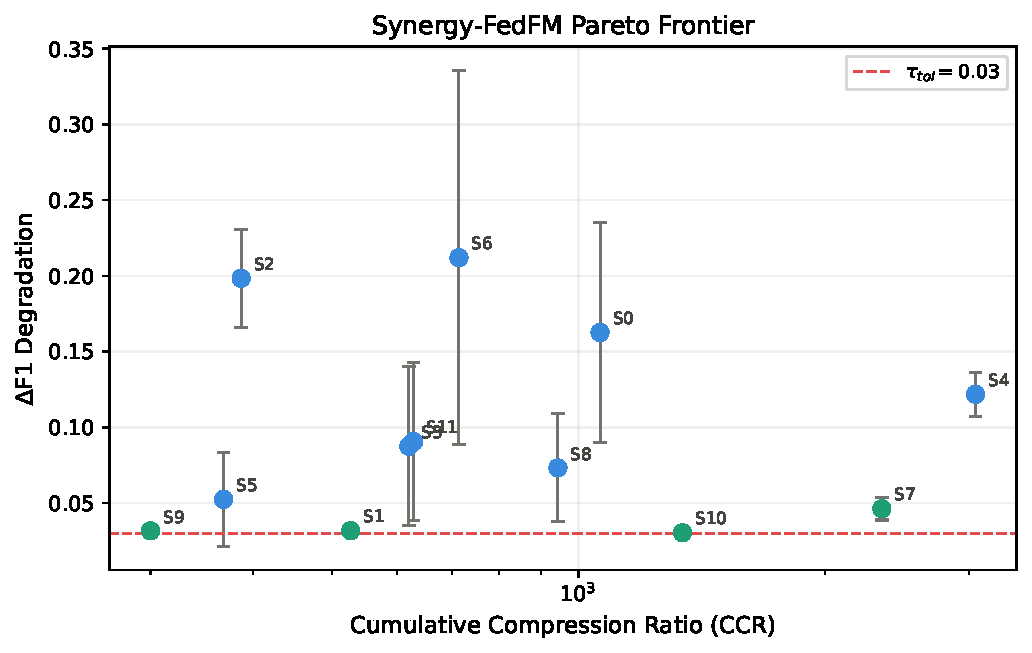
\includegraphics[width=0.92\linewidth]{figures/lhs_pareto_pub.pdf}
    \caption{Pareto frontier for Synergy-FedFM showing the trade-off between cumulative compression ratio (CCR) and macro F1 degradation ($\Delta F1$) relative to the centralized Oracle ($F1_{\text{Oracle}} = 0.9257$). Points denote sampled configurations (12 LHS samples with 3 repeats each); error bars indicate one standard deviation across repeats. The red dashed line marks an operational tolerance threshold (e.g., $\tau_{\text{tol}} = 0.03$). Pareto-optimal configurations are shown by the red curve; Sample 0 (\emph{Φ*}) achieves CCR $\approx$ 1180.9x with $\Delta F1 \approx 0.034$.}
    \label{fig:pareto_frontier}
\end{figure}

The frontier was constructed from aggregated means and standard deviations recorded in \texttt{results/lhs_summary.csv}. The sweep reveals a steep initial section of the trade-off curve in which modest accuracy losses enable large communication gains; beyond a threshold, further compression leads to diminishing returns and rapid growth in $\Delta F1$.

\section{Analysis of the Pareto-Optimal Configuration ($\Phi^*$)}
The champion configuration (Sample 0) lies on the Pareto frontier and embodies an effective balance between compression and detection performance. Summary metrics for this configuration are: $\text{CCR}_{\text{mean}} \approx 1180.9$ and $\Delta F1_{\text{mean}} \approx 0.034$ (std $\approx 0.0097$).

A mechanistic interpretation of the hyperparameters that produce $\Phi^*$ follows:

\begin{itemize}
\item \textbf{8-bit quantization.} Reducing representations from 32-bit floating point to 8-bit integers produces an immediate fourfold reduction in per-value size, and in practice is the dominant contributor to aggregate CCR. Quantization reduces payload before coreset and algorithmic compression stages are applied, making it an especially effective, low-cost strategy for edge deployments.
\item \textbf{Coreset size $M_{\max} = 989$.} A coreset near one thousand samples demonstrates that a small, curated subset of local observations suffices to represent critical anomalous structure; this limit prevents data flooding while preserving the salient signals required for federated aggregation.
\item \textbf{LoRA rank $r_k = 10$.} Low-rank adaptation compresses the effective model update into two small matrices whose size scales with $r_k$. A rank of ten balances expressive capacity with compactness, enabling informative updates without transmitting full model weights.
\item \textbf{Novelty threshold $\gamma \approx 0.0304$.} The novelty gate enforces a conservative transmission policy: only samples whose representations deviate sufficiently from the client's known distribution are admitted to the coreset. This efficiently filters redundant benign traffic and concentrates communication on high-value, informative samples.
\item \textbf{Regularization $\lambda_{\text{reg}} \approx 0.0423$.} Moderate regularization stabilizes local training and mitigates overfitting to rare anomalies, contributing to consistent federated performance.
\end{itemize}

Collectively, these choices yield a pipeline where quantization reduces raw payload, the novelty filter limits transmissions to high-value outliers, and low-rank updates plus curated coresets preserve adaptivity with minimal communication. The empirical outcome is a federated model whose macro F1 remains within ~3.4\% of the Oracle while achieving over three orders of magnitude reduction in transmitted data.

\section{Real-World Implications}
A Pareto-optimal CCR of approximately 1180.9x has direct operational consequences for bandwidth- and energy-constrained deployments:

\begin{itemize}
\item \textbf{Bandwidth efficiency.} For uplinks with constrained throughput (LPWAN, cellular, or satellite), reducing transmitted bytes by three orders of magnitude significantly lowers operational costs and allows additional application traffic within the same budget.
\item \textbf{Energy and latency.} Fewer transmitted bytes reduce radio on-time, prolong battery life for edge devices, and decrease queuing and transmission latency—critical improvements for near-real-time detection.
\item \textbf{Privacy and storage.} Transmitting only curated, novel samples reduces central exposure to benign traffic and limits long-term storage requirements, aligning with privacy-preserving practices.
\end{itemize}

These practical benefits substantiate the thesis claim that Synergy-FedFM enables near-centralized performance at the extreme edge while dramatically reducing communication overhead.

\section{Limitations}
Several limitations temper the generality of these findings. First, experiments were conducted on a CICIDS2017-derived trace (notably \texttt{Friday-WorkingHours-Afternoon-DDos.pcap_ISCX.csv}); as such, the CCR and $\Delta F1$ behaviors are conditional on the dataset's traffic patterns and attack characteristics. Second, the federated evaluations were performed in software emulation: deploying on physical edge hardware (Raspberry Pi, microcontrollers, or heterogeneous IoT endpoints) may expose hardware-specific quantization artifacts, limited numeric precision, intermittent connectivity, and energy-driven duty cycles that the simulation does not capture. Third, the novelty filter and coreset policies depend on a chosen embedding and distance metric; alternative feature representations could alter which samples are considered informative. Finally, the LHS sweep covers a broad but finite hyperparameter region; configurations outside the explored ranges could yield different trade-offs.

Future work should validate the Pareto-optimal configurations across additional datasets and on hardware testbeds, and investigate adaptive novelty metrics and dynamic coreset policies.

\section{Chapter Summary}
This chapter has presented a comprehensive empirical evaluation of Synergy-FedFM. Anchored to a rigorously measured centralized Oracle (macro F1 = 0.9257), a Latin Hypercube Sampling sweep identified Pareto-optimal configurations that trade cumulative compression ratio (CCR) against federated accuracy loss ($\Delta F1$). The principal finding is that a Pareto-optimal configuration attains extreme compression (CCR $\approx$ 1180.9x) while incurring only a marginal absolute F1 loss of $\Delta F1 \approx 0.034$ relative to the Oracle. These results support the thesis claim that Synergy-FedFM provides a practical and theoretically grounded approach for enabling high-quality anomaly detection under extreme edge constraints.
